% This file was created with tikzplotlib v0.10.1.
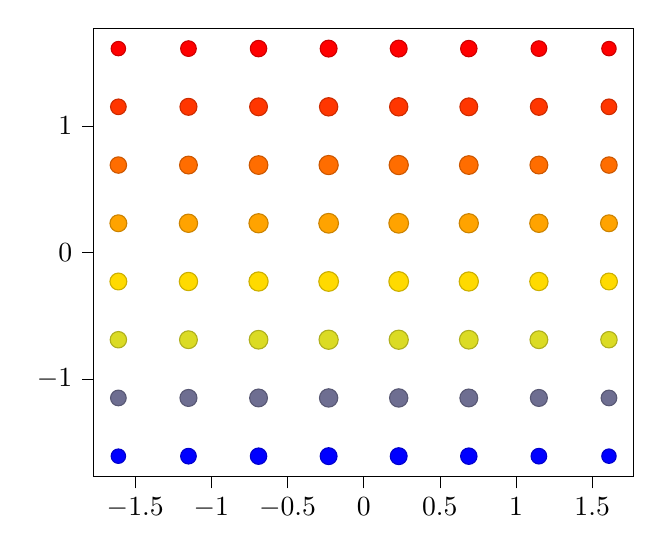
\begin{tikzpicture}

\definecolor{darkgray176}{RGB}{176,176,176}
\definecolor{steelblue31119180}{RGB}{31,119,180}

\begin{axis}[
tick align=outside,
tick pos=left,
x grid style={darkgray176},
xmin=-1.77135682106018, xmax=1.77135682106018,
xtick style={color=black},
y grid style={darkgray176},
ymin=-1.77135682106018, ymax=1.77135682106018,
ytick style={color=black}
]
\addplot [
  draw=steelblue31119180,
  fill=steelblue31119180,
  mark=*,
  only marks,
  scatter,
  scatter/@pre marker code/.append style={/tikz/mark size=\perpointmarksize},
  visualization depends on={\thisrow{sizedata} \as\perpointmarksize}
]
table{%
x  y  sizedata
-1.61032438278198 1.61032438278198 2.6057749
-1.15023183822632 1.61032438278198 2.8286114
-0.690139055252075 1.61032438278198 2.9655662
-0.230046361684799 1.61032438278198 3.0476043
0.230046361684799 1.61032438278198 3.0476043
0.690139055252075 1.61032438278198 2.9655662
1.15023183822632 1.61032438278198 2.8286114
1.61032438278198 1.61032438278198 2.6057749
-1.61032438278198 1.15023183822632 2.8286114
-1.15023183822632 1.15023183822632 3.070504
-0.690139055252075 1.15023183822632 3.2191706
-0.230046361684799 1.15023183822632 3.3082244
0.230046361684799 1.15023183822632 3.3082244
0.690139055252075 1.15023183822632 3.2191706
1.15023183822632 1.15023183822632 3.070504
1.61032438278198 1.15023183822632 2.8286114
-1.61032438278198 0.690139055252075 2.9655662
-1.15023183822632 0.690139055252075 3.2191706
-0.690139055252075 0.690139055252075 3.3750353
-0.230046361684799 0.690139055252075 3.468401
0.230046361684799 0.690139055252075 3.468401
0.690139055252075 0.690139055252075 3.3750353
1.15023183822632 0.690139055252075 3.2191706
1.61032438278198 0.690139055252075 2.9655662
-1.61032438278198 0.230046361684799 3.0476043
-1.15023183822632 0.230046361684799 3.3082244
-0.690139055252075 0.230046361684799 3.468401
-0.230046361684799 0.230046361684799 3.564349
0.230046361684799 0.230046361684799 3.564349
0.690139055252075 0.230046361684799 3.468401
1.15023183822632 0.230046361684799 3.3082244
1.61032438278198 0.230046361684799 3.0476043
-1.61032438278198 -0.230046361684799 3.0476043
-1.15023183822632 -0.230046361684799 3.3082244
-0.690139055252075 -0.230046361684799 3.468401
-0.230046361684799 -0.230046361684799 3.564349
0.230046361684799 -0.230046361684799 3.564349
0.690139055252075 -0.230046361684799 3.468401
1.15023183822632 -0.230046361684799 3.3082244
1.61032438278198 -0.230046361684799 3.0476043
-1.61032438278198 -0.690139055252075 2.9655662
-1.15023183822632 -0.690139055252075 3.2191706
-0.690139055252075 -0.690139055252075 3.3750353
-0.230046361684799 -0.690139055252075 3.468401
0.230046361684799 -0.690139055252075 3.468401
0.690139055252075 -0.690139055252075 3.3750353
1.15023183822632 -0.690139055252075 3.2191706
1.61032438278198 -0.690139055252075 2.9655662
-1.61032438278198 -1.15023183822632 2.8286114
-1.15023183822632 -1.15023183822632 3.070504
-0.690139055252075 -1.15023183822632 3.2191706
-0.230046361684799 -1.15023183822632 3.3082244
0.230046361684799 -1.15023183822632 3.3082244
0.690139055252075 -1.15023183822632 3.2191706
1.15023183822632 -1.15023183822632 3.070504
1.61032438278198 -1.15023183822632 2.8286114
-1.61032438278198 -1.61032438278198 2.6057749
-1.15023183822632 -1.61032438278198 2.8286114
-0.690139055252075 -1.61032438278198 2.9655662
-0.230046361684799 -1.61032438278198 3.0476043
0.230046361684799 -1.61032438278198 3.0476043
0.690139055252075 -1.61032438278198 2.9655662
1.15023183822632 -1.61032438278198 2.8286114
1.61032438278198 -1.61032438278198 2.6057749
};
\end{axis}

\end{tikzpicture}
